
\chapter{Rare Linguistic Styles: Robustness to Language Alternation}
\label{ch:robustness}




\begin{comment}

 %Neural machine translation (NMT) 
 NMT models have progressed from research prototypes to production systems and have enabled communication across language barriers. 
 %NMT also allowed scaling to hundreds of languages, supporting multilingual translations.
 %Multilingual NMT is an attractive way to increase language coverage, as it enables a single model to support hundreds of languages.
 Multilingual humans can and do seamlessly switch back and forth between languages when communicating. 
 However, multilingual (machine) translation models are not robust to such sudden changes.
 In this chapter, we explore the robustness of multilingual MT models to language switching and propose checks to measure switching capability. 
 We also investigate simple and effective data augmentation methods that can enhance robustness. A glass-box analysis of attention modules demonstrates the effectiveness of these methods in improving robustness.

\end{comment}

%\section{Introduction}

%Neural machine translation (NMT)~\cite{sutskever2014seq2seq,bahdanau2014nmtattn,vaswani-2017-attention}

NMT has made significant progress, from supporting only a pair of languages per model to now simultaneously supporting up to hundreds of languages \cite{johnson-etal-2017-googleNMT,zhang-etal-2020-multiling-nmt,tiedemann-2020-tatoeba,gowda2021-many-eng}. 
Multilingual NMT models have been deployed in production systems and are actively used to translate across languages in day-to-day settings \cite{wu-etal-2016-GNMT,turovsky-2017-googletrans,mohan-2021-ms-translator}. 
%Human evaluation of MT models, although desirable, is expensive and slow. 
%Hence MT models are often evaluated using automatic evaluation metrics on held-out datasets.
%The held-out sets, just like the training datasets, contain segmented sentences as input, and (one or more) human translated segments as references. 
A great many metrics for evaluation of machine translation have been proposed \cite{papineni-etal-2002-bleu,doddington-2002-NIST,banerjee-lavie-2005-meteor,snover2006TER,popovic-2015-chrf,lo-2019-yisi}, including \maf1 in Chapter~\ref{ch:eval-metrics}, however nearly all approaches consider translation in the context of a \textit{single sentence}. Even the approaches that generalize to support translation of multiple languages \cite{zhang-etal-2020-multiling-nmt,tiedemann-2020-tatoeba,gowda2021-many-eng} continue to use the single-sentence paradigm. In reality, however, multilingual environments involve switching between languages and scripts.
For instance, the European Parliament\footnote{\url{https://www.europarl.europa.eu/doceo/document/CRE-9-2021-11-10_EN.pdf}}
and Parliament of India\footnote{\url{https://web.archive.org/web/20220105061052/http://loksabhadocs.nic.in/debatestextmk/17/VII/01.12.2021.pdf}} hold debates in multilingual environments where speakers seamlessly switch languages.


Language Alternation, also known as code switching (CS), is a linguistic phenomenon in which the speaker alternate between two or more languages in the context of a single conversation \cite{cms-and-ury-1977-biling}. 
CS is further classified into two major categories: (1) intersentential, where switching happens at sentence or clause boundaries, and (2) intra-sentential, where the switching happens within a sentence or clause.  
\citet{myers1989codeswitching} argues that \textit{distinction between inter- and intra-sentential switching is poorly motivated, and both can occur as part of the same conversation turn}. An example CS between two Indian languages having both inter- and intra-sentential switching is given in Figure~\ref{fig:example-langswitch-hinkan}.
CS has been studied extensively in linguistics communities \cite{nilep-2006-codeswitch}; 
however, the efforts in MT community is sparse \cite{gupta-etal-2021-training}, which we attempt to address in this chapter.

%The reasons why the speakers chose to alternate between languages is extensively studies by social sciences communities, and is beyond the scope of this work. 

% \footnote{Credits: Twitter Inc. Tweet URL: \url{https://twitter.com/PMOIndia/status/1481605615739084800}}
%\begin{figure}[t]
%    \centering
%    
\includegraphics[width=\linewidth]{pmi-tweet-langswitch.png}
%    \caption{A tweet demonstrating language switching between English and Hindi; such seamless language switching is common in multilingual environments.}
%    \label{fig:example-langswitch}
%\end{figure}


\begin{figure}[ht]
    \centering
    \renewcommand{\arraystretch}{1.4}
    \begin{tabular}{ p{0.95\linewidth}}
    \hline
    Original: {``\textsf{bandaaginda bari} \textit{bageeche ke bahar}\textsf{-e iddivi.} \textit{kahaani ke andhar} \textsf{ bandu bidona.} \textit{kaam bolo saab.}"} \\ 
    \hdashline
    \textsf{Kannada: ``bandaaginda bari vishayada horagadene iddivi. katheya olagade bandu bidona. kelasa heli saar."}\\
    %\textcolor{OliveGreen}{Hindi: ``.''}\\
    English Translation:  ``From the time I've reached here, we've stayed outside of the topic. Let's come into the matter. Tell me the work, sir."\\
    \hline
    \end{tabular}
    \caption{Demonstration of language switching between \textsf{Kannada} and \textit{Hindi}.
    The original dialogue is taken from an Indian movie. Such seamless language switching is common among multilingual speakers.}
    \label{fig:example-langswitch-hinkan}
    
    
    \begin{comment}
    \vspace{5mm}
    \begin{tabular}{ p{0.95\linewidth}}
    \hline
    Original: \textit{``\textcolor{blue}{Ce moment} \textcolor{OliveGreen}{when you start} \textcolor{blue}{penser en deux langues} \textcolor{OliveGreen}{at the same} \textcolor{blue}{temps!}"} \\
    \textcolor{blue}{French: ``Ce moment quand vous commencez à penser en deux langues au même temps!"}\\
    \textcolor{OliveGreen}{English: ``The moment when you start to think in two languages at the same time!"}\\
    \hline
    \end{tabular}
    \caption{Demonstration of language switching between \textcolor{blue}{French} and \textcolor{OliveGreen}{English}.}
    \end{comment}
\end{figure}



In this chapter, we show that, multilingual NMT models, as commonly built, are \textit{not robust} to multi-sentence translation, especially when language switching is involved. The contributions of this chapter are outlined as follows:
Firstly, inspired by \textsc{CheckList}~\cite{ribeiro-etal-2020-beyond}, a few simple but effective checks for improving the test coverage in multilingual NMT evaluation are described (Section~\ref{sec:multiling-mt-checks}).
Secondly, we explore training data augmentation techniques such as concatenation and noise addition in the context of multilingual NMT (Section~\ref{sec:train-aug}).
Third, using a many-to-one multilingual translation task setup (Section~\ref{sec:setup}), we investigate the relationship between training data augmentation methods and their impact on multilingual test cases. 
Fourth, we conduct a glass-box analysis of cross-attention in the Transformer architecture and show visually as well as quantitatively that the models trained with concatenated training sentences learn a more sharply focused attention mechanism than others.
% \mg{Per Jon's comment, it can be replaced with ``more sharply focused''}(Section~\ref{sec:attn-bleed}).
Finally, we examine how our data augmentation strategies generalize to multi-sentence translation for a variable number of sentences, and determine that two-sentence concatenation in training is sufficient to model many-sentence concatenation in inference (Section~\ref{sec:generalization}). 

%\section{Language Alternation}
%\tg{TODO: write about language alternation. different kinds. why it is important. why it is challenging.}


%%%%%%%%%%%%%%%%%%%%%%%%%%SECTION%%%%%%%%%%%%%%%%%%%%%%%%%%%%%%%%%%%
\section{Multilingual Translation Evaluation: Additional Checks}
\label{sec:multiling-mt-checks}

Inspired by the behavior testing paradigm in software engineering, \citet{ribeiro-etal-2020-beyond} propose a \textsc{CheckList} to test beyond the accuracy of NLP models.
The central idea of \textsc{CheckList} is that given any held-out set, one can improve the coverage of testing by modifying the set in a systematic way designed to test linguistic capabilities of natural language processing (NLP) modeling.
Some of the modifications \textsc{CheckList} employs are: synonym replacement, named entity replacement, negation, etc. 
Although these modifications are straightforward in tasks such as sentiment classification, such modifications on parallel sentences while maintaining the consistency on both sides is not trivial.
%are non-trivial in machine translation between varieties of languages.
%For instance, 
Nevertheless, the principles of behavior testing and their application to improve test coverage in machine translation are intriguing. 
We, therefore, explore suitable checks in the context of multilingual NMT. 

\textit{Definitions:} Translation tasks are categorized as \textit{bilingual} if a single source language is translated to a single target language, and \textit{multilingual} if two or more languages are on either of the source or target side. Multilingual tasks are further sub-classified based on the number of languages and the side they on are as many-to-one, one-to-many, and many-to-many. 
In this chapter, we focus on many-to-one (i.e., many source languages, one target) multilingual translation.

\textit{Notation:} For simplicity, consider a many-to-one model that translates sentences from $K$ source languages,  $\{L_k | k = 1, 2, ... K\}$, to a target language, $T$.
Let $x_{i}^{(L_k)}$ be a sentence in the source language $L_k$, and let its translation in the target language be $y_{i}^{(T)}$; where unambiguous, we omit the superscripts.

We propose the following checks to be used for multilingual NMT:
%  refer to Table~\ref{tab:test-aug} for a summary
\begin{description}[itemsep=-2mm,topsep=0mm,leftmargin=3mm]
    
    \item[C-SL:] Concatenate consecutive sentences in the same language. 
    It is not always trivial to determine sentence segmentation in continuous language. This check thus tests if the model is invariant to a missed segmentation. 
    This check is possible iff held-out set sentence order preserves the coherency of the original document. 
    %\code{(x$_{i}$ ␣ x$_{i+1}$) $\rightarrow$ (y$_{i}$ ␣ y$_{i+1}$)}
    Formally, $$x^{(L_k)}_{i} + x^{(L_k)}_{i+1} \rightarrow y_i + y_{i+1}$$
    
    In practice, we use a space character to join sentences, indicated by the concatenation operator `$+$'.\footnote{We focus on orthographies that use space as a word-breaker.
    In orthographies without a word-breaker, joining may be performed without any glue character.}
    \item[C-TL:] Consecutive sentences in the source and target languages.
    This check tests if the MT system can preserve phrases that are already in the target language, and if the MT system can translate in the presence of code and language switching settings. For completeness, we can test both source-to-target and target-to-source language switching, as follows:
    \begin{align*}
       x^{(L_k)}_i + y_{i+1} & \rightarrow y_i + y_{i+1} \\
       y_{i} + x^{(L_k)}_{i+1} & \rightarrow y_{i} + y_{i+1}
    \end{align*}
Similar to C-SL, this check also requires the held-out set sentence order to preserve the coherency of the original document.
    %Similar to do-not-translate. Tests if model detects target language and preserves it. Assumption: test sentence preserves original document order.\\
    %\code{(x$_{i}$  ␣ y$_{i+1}$) $\rightarrow$ (y$_{i}$  ␣ y$_{i+1}$)} \\
    %\code{(y$_{i-1}$ ␣ x$_{i}$) $\rightarrow$ (y$_{i-1}$ ␣  y$_{i}$)}
    
    \item[C-XL:] This check tests if a multilingual MT system is agnostic to language switching. 
    This check is created by concatenating consecutive sentences across source languages. 
    This is possible iff the held-out sets are multi-parallel across languages, and, similar to the previous two, each preserves the coherency of the original documents.
    Given two languages $L_k$ and $L_m$, we obtain a test sentence as follows: 
    $$x^{(L_k)}_i + x^{(L_m)}_{i+1} \rightarrow y_i + y_{i+1}$$
    
    \item[R-XL:] This check tests if a multilingual MT system can function in light of a topic switch among its supported source languages. 
    % \mg{is competence the actual intended word here? what does competence languages mean?}
    For any two languages $L_k$ and $L_m$ and random positions $i$ and $j$ in their original corpus, we obtain a test segment by concatenating them as: 
    $$ x^{(L_k)}_i + x^{(L_m)}_j \rightarrow y_i + y_j $$
     This method makes the fewest assumptions about the nature of held-out datasets, i.e., unlike previous methods, neither multi-parallelism nor coherency in sentence order is necessary.
 \end{description}
 
 %For each of the above augmentations, its reference sentence is obtained by concatenating the corresponding parallel counterparts in the target language. 

%%%%========== COMMENT==========
\begin{comment}  
\begin{table}[htb]
\centering
\renewcommand{\arraystretch}{1.5}
\begin{tabular}{l l l }
\hline
    \textbf{Name} & \textbf{Source} & \textbf{Target} \\ 
\hline
    C-SL & $x^{(L_k)}_{i} + x^{(L_k)}_{i+1}$ & $y_i + y_{i+1}$ \\ \hdashline
\multirow{2}{*}{C-TL} & $x^{(L_k)}_i + y_{i+1}$ & $y_i + y_{i+1}$ \\
     & $y_{i-1} + x^{(L_k)}_{i}$ & y$_{i-1} + y_{i}$ \\ \hdashline
    C-XL & $x^{(L_k)}_i + x^{(L_m)}_{i+1}$ & $y_i + y_{i+1}$ \\
    R-XL & $x^{(L_k)}_i + x^{(L_m)}_j$ & $y_i + y_j$ \\
\hline
\end{tabular}
\caption{Held-out dataset augmentation methods. The operator `$+$' is concatenation with a space character.}
\label{tab:test-aug}
\end{table}
\end{comment}
%%%%========== COMMENT==========


%%%%%%%%%%%%%%%%%%%%%%%%%%SECTION%%%%%%%%%%%%%%%%%%%%%%%%%%%%%%%%%%%
\section{Improving Robustness via Data Augmentation Methods}
\label{sec:train-aug}
In the previous section, we described several ways of improving \textit{test} coverage for multilingual translation models.
In this section, we explore \textit{training} data augmentation techniques to improve robustness to language switching settings.

\subsection{Concatenation}
Concatenation of training sentences has been proven to be a useful data augmentation technique; \citet{nguyen-etal-2021-data} investigate key factors behind the usefulness of training segment concatenations in \textit{bilingual} settings. 
Their experiments reveal that concatenating random sentences performs as well as consecutive sentence concatenation, which suggests that discourse coherence is unlikely the driving factor behind the gains.
They attribute the gains to three factors: context diversity, length diversity, and position shifting.

In this chapter, we investigate training data concatenation under \textit{multilingual} settings, hypothesizing that concatenation helps achieve the robustness checks that are described in the prior section. Our training concatenation approaches are similar to our check sets, with the notable exception that we do not consider consecutive sentence training specifically, both because of \citet{nguyen-etal-2021-data}'s finding and because training data gathering techniques can often restrict the availability of consecutive data \cite{banon-etal-2020-paracrawl}.  
We investigate the following sub-settings for concatenations:

\begin{description}[itemsep=0.5mm,topsep=0pt,leftmargin=5mm]
\item[CatSL:] Concatenate a pair of source sentences in the same language, using space whenever appropriate (e.g. languages with space separated tokens). 
%\code{(x$_i$ ␣ x$_j$) $\rightarrow$ (y$_i$ ␣ y$_j$)} where \code{x$_i$} and \code{x$_i$} are in the same language.
$$x^{(L_k)}_i + x^{(L_k)}_j \rightarrow y_i + y_j$$

\item[CatXL:] Concatenate a pair of source sentences, without constraint on language.
%\code{(x$_i$ ␣ x$_j$) $\rightarrow$ (y$_i$ ␣ y$_j)$} where $x_i$ and $x_j$ are not necessarily in the same language.
$$x^{(L_k)}_i + x^{(L_m)}_j \rightarrow y_i + y_j$$
\item[CatRepeat:] The same sentence is repeated and then concatenated. 
Although this seems uninteresting, it serves a key role in ruling out gains possibly due to data repetition and modification of sentence lengths.
%\code{(x$_i$ ␣ x$_i$) $\rightarrow$ (y$_i$ ␣ y$_i$)}
 $$x^{(L_k)}_i + x^{(L_k)}_i \rightarrow y_i + y_i$$
\end{description}

%Refer to Table~\ref{tab:train-aug} for an overview of these methods.
\subsection{Adding Noise}
We hypothesize that introducing noise during training might help achieve robustness, and investigate two approaches that rely on noise addition:
\begin{description}[itemsep=0.5mm,topsep=0pt,leftmargin=5mm]
\item[DenoiseTgt:] Form the source side of a target segment by adding noise to it. 
% \texttt{noise(y) $\rightarrow$ y}
Formally, $$noise(y; r) \rightarrow y$$ where, hyperparameter $r$ controls the noise ratio.
Denoising is an important technique in unsupervised NMT \cite{Artetxe-2018-unmt-iclr,Lample-2018-unmt-iclr}.

\item[NoisySrc:] Add noise to the source side of a translation pair.
% \code{noise(x) $\rightarrow$ y}
Formally, $$noise(x; r) \rightarrow y$$ 
This resembles back-translation~\cite{sennrich-etal-2016-improving} where augmented data is formed by pairing noisy source sentences with clean target sentences.

%\item[RevSrc:] Reverse the words in source segment and use it as input while the target is unmodified. 
% \code{reverse(y) $\rightarrow$ y}
% \code{reverse(x) $\rightarrow$ y}
%\item[RevTgt:]  Reverse the words in target segment and use it as input while target side is unmodified segment.
\end{description}

%Refer to Table~\ref{tab:train-aug} for an overview of these methods.
%Both RevSrc and RevTgt reverses word order while preserving the character order within words.
The function $noise(...; r)$ is implemented as follows: %for a given $r \in (0, 100)$, 
(i) $r\%$ of random tokens are dropped, 
(ii) $r\%$ of random tokens are replaced with random types uniformly sampled from vocabulary, and 
(iii) $r\%$ of random tokens' positions are displaced within a sequence.
We use $r=10\%$ in the experiments discussed in this chapter.

\begin{comment} %=======COMMENT=====
\begin{table}[htb]
\centering
\renewcommand{\arraystretch}{1.3}
\begin{tabular}{l l l}
\hline
    \textbf{Name}   & \textbf{Source} & \textbf{Target} \\
\hline
    CatSL      & $x^{(L_k)}_i + x^{(L_k)}_j$ & $y_i + y_j$ \\
    CatXL      & $x^{(L_k)}_i + x^{(L_m)}_j$ & $y_i + y_j$ \\
    CatRepeat  & $x^{(L_k)}_i + x^{(L_k)}_i$ & $y_i + y_i$ \\ \hdashline
    NoisySrc   & $noise(x)$ & $y$ \\
    DenoiseTgt & $noise(y)$ & $y$ \\
    %RevSrc     & $rev\_words(x)$ & $y$ \\    
    %RevTgt     & $rev\_words(y)$ & $y$ \\
\hline
\end{tabular}
\caption{Training data augmentation methods; Operator `$+$' is concatenation with a space character. }
\label{tab:train-aug}
\end{table}
%%% \ end{comment}

%\begin{comment}  % ==== COMMENT
\end{comment} 
%=======COMMENT=====


\renewcommand{\arraystretch}{1.2}
\begin{table}[htb]
    \centering
\begin{tabular}{l @{\hspace{6pt}} c @{\hspace{6pt}} r }
\hline
\textbf{Language} & \textbf{In-domain} & \multicolumn{1}{c}{\textbf{All-data}} \\
\hline
Bengali (BN)  & 23.3k/0.4M/0.4M    & 1.3M/19.5M/21.3M \\
Gujarati (GU) & 41.6k/0.7M/0.8M    & 0.5M/07.2M/09.5M \\
Hindi (HI)    & 50.3k/1.1M/1.0M    & 3.1M/54.7M/51.8M \\
Kannada (KN)  & 28.9k/0.4M/0.6M    & 0.4M/04.6M/08.7M \\
{Malayalam}(ML) & 26.9k/0.3M/0.5M  & 1.1M/11.6M/19.0M \\
Marathi (MR)  & 29.0k/0.4M/0.5M    & 0.6M/09.2M/13.1M \\
Oriya (OR)    & 32.0k/0.5M/0.6M    & 0.3M/04.4M/05.1M \\
Punjabi (PA)  & 28.3k/0.6M/0.5M    & 0.5M/10.1M/10.9M \\
Tamil (TA)    & 32.6k/0.4M/0.6M    & 1.4M/16.0M/27.0M \\
Telugu (TE)   & 33.4k/0.5M/0.6M    & 0.5M/05.7M/09.1M \\
\hdashline
All   & 326k/5.3M/6.1M     & 9.6M/143M/175M\\ 
\hline
\end{tabular} 
    \caption{Training dataset statistics: \textit{segments / source / target tokens}, before tokenization.}
    \label{tab:training-stats}
%\end{table}
\vspace{5mm}
%\begin{table}[htb]
    \centering
\begin{tabular}{l c c}
\hline
\textbf{Name} & \textbf{Dev} & \textbf{Test} \\
\hline
Orig & 10k/140.5k/163.2k & 23.9k/331.1k/385.1k \\
C-SL & 10k/281.0k/326.4k & 23.9k/662.1k/770.1k \\
C-TL & 10k/303.7k/326.4k & 23.9k/716.1k/770.1k \\
C-XL & 10k/283.9k/326.4k & 23.9k/670.7k/770.1k \\
R-XL & 10k/216.0k/251.2k & 23.9k/514.5k/600.5k \\
\hline
\end{tabular}
    \caption{Development and test set statistics: \textit{segments / source / target tokens}, before tokenization. 
    The row named `Orig' is the union of all ten individual languages' datasets, and the rest are created as per definitions in Section~\ref{sec:multiling-mt-checks}.
    Dev-Orig set is used for validation and early stopping in all our multilingual models.}
    \label{tab:heldout-stats}
\end{table}


\begin{table}[htb]
    \centering
    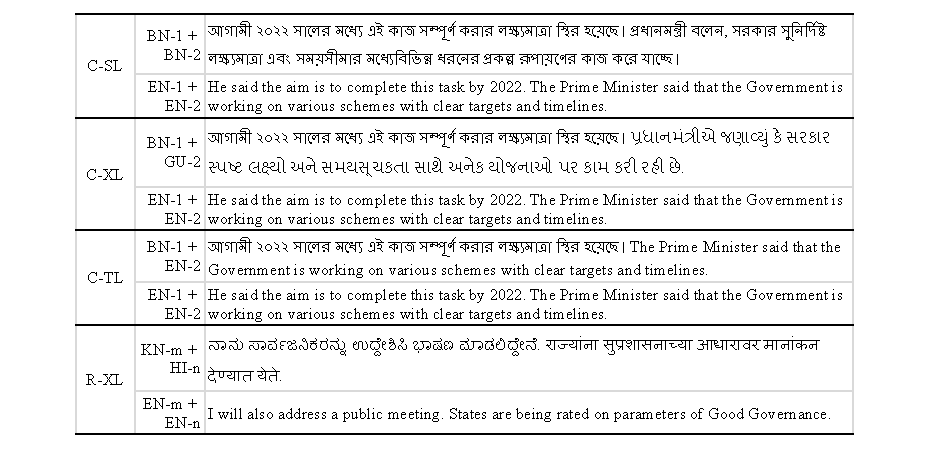
\includegraphics[width=0.99\linewidth,trim={12mm 2mm 12mm 2mm},clip]{img/robustness/example-concat-devs.pdf}
    \caption{Concatenated sentence examples from the development set. 
    Bengali (BN), Gujarati (GU), Kannada (KN), and Hindi (HI) are chosen for illustrations; similar augmentations are performed for all other languages in the corpus.
    Indices $1$ and $2$ indicate consecutive positions, and $m$ and $n$ indicate random positions.}
    \label{tab:dev-aug-example}
\end{table}

%%%%%%%%%%%%%%%%%%%%%%%%%%SECTION%%%%%%%%%%%%%%%%%%%%%%%%%%%%%%%%%%%
\section{Setup}
\label{sec:setup}

\subsection{Dataset}
\label{ch:rtobustness-sec:dataset}
We use publicly available datasets from The Workshop on Asian Translation 2021 (WAT21)'s  \textit{MultiIndicMT}~\cite{nakazawa-etal-2021-overview}\footnote{\url{http://lotus.kuee.kyoto-u.ac.jp/WAT/indic-multilingual/}} shared task. This task involves translation between English(EN) and 10 Indic Languages, namely: Bengali(BN), Gujarati(GU), Hindi(HI), Kannada(KN), Malayalam(ML), Marathi(MR), Oriya(OR), Punjabi(PA), Tamil(TA) and Telugu(TE). 
The development and held-out test sets are multi-parallel and contain 1,000 and 2,390 sentences, respectively. 
The training set contains a small portion of data from the same domain as the held-out sets, as well as additional datasets from other domains.
All the training data statistics are given in Table~\ref{tab:training-stats}.
We focus on the Indic$\shortarrow$English (many-to-one) translation direction in this chapter.

Following the definitions in Section~\ref{sec:multiling-mt-checks}, we create C-SL, C-TL, C-XL, and R-XL versions of development and test sets; statistics are given in Table~\ref{tab:heldout-stats}. 
An example demonstrating the nuances in all these four methods is shown in Table~\ref{tab:dev-aug-example}. 
Following the definitions in Section~\ref{sec:train-aug}, we create CatSL, CatXL, CatRpeat, DenoiseTgt, and NoisySrc augmented training segments. 
For each of these training corpus augmentation methods, we restrict the total augmented sentences to be roughly the same number of segments as the original corpus, i.e., 326k and 9.6M segments in the in-domain and the all-data setup, respectively.


\subsection{Model and Training Process}

We use a Transformer base model \cite{vaswani-2017-attention}, similar to the one used in Chapter~\ref{ch:nlg-imbalance}, having 512 hidden dimensions, 6 encoder and decoder layers, 8 attention heads, and intermediate feedforward layers of 2048 dimensions.
We use our PyTorch based NMT toolkit (Section~\ref{sec:rtg}).
% named RTG \cite{gowda-etal-2021-many} to train all our models.\footnote{\url{https://isi-nlp.github.io/rtg/}}.
As described in Chapter~\ref{ch:nlg-imbalance}, tuning the vocabulary size and batch size are important to achieve competitive performance.
We use byte-pair-encoding (BPE) \cite{sennrich-etal-2016-bpe}, with vocabulary size adjusted as per our findings in Chapter~\ref{ch:nlg-imbalance}. %, except, to avoid extremely large vocabularies which are infeasible in practice, we place a maximum limit of 500k and 128k types on source and target, respectively\footnote{Largest vocabulary sizes found are 230k and 63k}.
Since the source side has many languages and the target side has only a single language, we use a larger source vocabulary than that of the target.
The source side vocabulary contains BPE types from all 11 languages (i.e., ten source languages and English), whereas to improve the efficiency in the decoder's softmax layer, the target vocabulary is restricted to contain English only. 
Our in-domain limited-data setup learns BPE vocabularies of 30.4k and 4.8k types for source and target languages.
Similarly, the all-data setup learns 230.4k and 63.4k types.
The training batch size used for all our multilingual models is 10k tokens for the in-domain limited-data setup, and 25k tokens for the larger all-data setup.
The batch size for the baseline bilingual models is adjusted as per data sizes using \textit{`a thousand per million tokens'} rule of thumb that we have come to devise with a maximum of 25k tokens.
% \mg{citation for this?}\tg{no citation available; this is something I found while redoing NMT Learning curve (V2) that never got published}.
 The median sequence lengths in training after subword segmentation but before sentence concatenation are 15 on the Indic side and 17 on the English side. 
 We model sequence lengths up to 512 time steps during training.
%i.e., for a dataset having \code{w} target language tokens, the adjusted batch size is as per (Python) function: \code{min(25000, round(w/1000, -3))}.
We use the same learning rate schedule as \citet{vaswani-2017-attention}.
We train our models until a maximum of 200k optimizer steps, and use early stopping with patience of 10 validations.
Validations are performed after every 1000 optimizer steps.
All our models are trained using one Nvidia A40 GPU per setting. 
The smaller in-domain setup takes less than 24 hours per run, whereas the larger all-data setup takes at most 48 hours per run (or less when early stopping criteria are reached).
We run each experiment two times and report the average. During inference, we average the last 5 checkpoints and use a beam decoder of size 4 and length penalty of $\alpha=0.6~$\cite{vaswani-2017-attention,wu-etal-2016-GNMT}. 


\begin{table*}[h!t]
\centering
%\small
\setlength{\tabcolsep}{4pt}
\begin{tabular}{l | rr | rrrrr rrrrr}
\hline
& Dev & Test & BN & GU & HI & KN & ML & MR & OR & PA & TA & TE \\
\hline
{WAT21 biling indomain~\ddag} & & 18.6 & 11.3 & 26.2 & 28.2 & 20.3 & 13.6 & 15.1 & 16.4 & 23.7 & 16.1 & 14.7 \\
{Biling; indomain~\ddag} & 24.1 & 21.6 & 13.2 & 29.3 & 32.9 & 22.7 & 17.9 & 16.9 & 16.4 & 27.4 & 18.1 & 21.0 \\ \hdashline 
{Biling; indomain} & 23.9 & 21.5 & 13.1 & 29.2 & 32.6 & 22.5 & 17.7 & 16.8 & 16.4 & 27.3 & 18.0 & 20.9 \\
{Many-to-one; indomain} & 26.5 & 22.7 & 18.7 & 25.7 & 27.8 & 23.1 & 21.2 & 20.8 & 21.1 & 25.8 & 20.6 & 22.4 \\
{Many-to-one; all data} & 35.0 & 32.4 & 26.2 & 36.8 & 40.1 & 31.7 & 30.0 & 29.8 & 30.5 & 38.8 & 29.1 & 30.8 \\ 
\hline
\end{tabular} 
\caption{Indic$\shortarrow$English BLEU scores.
Rows indicated by \ddag{} match the evaluation settings used by WAT21 shared task (i.e., tokenized BLEU). 
The rows without \ddag{} are detokenized BLEU obtained from \textsc{SacreBLEU} \cite{post-2018-sacrebleu}. 
Dev and Test are average across 10 languages.
}
\label{tab:bleu-base}
\end{table*}

%\vspace{2mm}
%\renewcommand{\arraystretch}{1.2}
\begin{table*}[htb]
\centering
%\small
\setlength{\tabcolsep}{4pt}
\begin{tabular}{l l rrrrr : rrrrr}
\hline
& & \multicolumn{5}{c:}{\textbf{Dev}} & \multicolumn{5}{c}{\textbf{Test}} \\
ID & In-domain & Avg & C-TL & C-SL & C-XL & R-XL & Avg & C-TL & C-SL & C-XL & R-XL \\
\hline
\#I1 & Baseline (B)            & 26.5 & 10.8 & 17.0 & 16.9 & 15.9               & 22.7 & 9.4 & 14.9 & 14.7 & 13.6 \\
\hdashline
\#I2 & B+CatRepeat & 25.3 & 9.9 & 14.5 & 14.7 & 13.3 & 21.6               & 8.6 & 13 & 13 & 11.4 \\ 
\#I3 & B+CatXL     & 26.2 & 12.6 & 26.1 & 25.9 & \textbf{26.5} & 22.6 & 11.1 & 22.7 & 22.5 & 22.3 \\
\#I4 & B+CatSL     & 26.1 & 13.2 & 26.1 & 25.9 & \textbf{26.5} & 22.6 & 11.4 & 22.9 & \textbf{22.6} & 22.3 \\
\#I5 & B+NoisySrc  & 25.2 & 10.5 & 16.2 & 16.0 & 15.2               & 21.2 & 9.1 & 14.3 & 14.1 & 12.9 \\
\#I6 & B+DenoiseTgt & \textbf{26.7} & 40.4 & 17.9 & 17.7 & 16.6    & \textbf{23.2} & {39.7} & 15.7 & 15.4 & 14.1 \\
%G & b+DenoiseTgtExt  & 26.5 & \hl{43.9} & 17.9 & 17.8 & 16.4          & 23.0 & \hl{42.8} & 15.8 & 15.5 & 14.2 \\
%H & b+RevSrc           & 24.6 & 8.7 & 15.1 & 15.0 & 14.1                & 21.0 & 7.4 & 13.3 & 13.1 & 12.0 \\
%I & b+RevTgt           & \hl{27.0} & 19.6 & 18.0 & 17.8 & 16.8          & \hl{23.4} & 18.4 & 15.9 & 15.6 & 14.3 \\
\hdashline
\#I7 & B+CatXL+DenoiseTgt & 26.1 & \textbf{55.2} & \textbf{26.3} & \textbf{26.0} & 26.4 & 22.6 & \textbf{53.4} & \textbf{23.0} & \textbf{22.6} & \textbf{22.4} \\ 
\hline
\end{tabular} 
\caption{ Indic$\shortarrow$English BLEU scores for models trained on in-domain training data only. The best scores are shown in bold. }
\label{tab:bleu-indom-aug}
%\end{table*}
\vspace{2mm}
%\begin{table*}[htb]
%    \centering
%    \small
\begin{tabular}{l l rrrrr : rrrrr}
\hline
& & \multicolumn{5}{c:}{\textbf{Dev}} & \multicolumn{5}{c}{\textbf{Test}} \\
ID & All-data & Avg & C-TL & C-SL & C-XL & R-XL & Avg & C-TL & C-SL & C-XL & R-XL \\
\hline
\#A1 & Baseline (B) & \textbf{35.0} & 43.1 & 30.0 & 29.5 & 28.2 & \textbf{32.4} & 42.2 & 27.8 & 27.3 & 26.1 \\
\hdashline
\#A2 & B+CatRepeat & 34.5 & 43.7 & 30.3 & 29.9 & 28.8 & 32.0 & 42.9 & 28.0 & 27.6 & 26.3 \\ 
\#A3 & B+CatXL  & 34.1 & 53.3 & 31.9 & \textbf{33.7} & \textbf{34.4} & 31.6 & 52.4 & 29.7 & \textbf{31.0} & \textbf{31.2} \\
\#A4 & B+CatSL & 33.6 & 54.0 & \textbf{32.5} & 32.2 & 34.3 & 31.3 & 53.3 & \textbf{30.4} & 29.9 & 31.1 \\
\#A5 & B+NoisySrc & 34.9   & 42.1 & 29.8 & 29.2 & 27.8 & 32.3 & 41.7 & 27.6 & 27.1 & 25.8 \\
\#A6 & B+DenoiseTgt      & 33.3 & 60.0 & 28.9 & 28.4 & 27.3 & 31.3 & 59.4 & 27.1 & 26.5 & 25.4 \\
%G & b+DenoiseTgtExt   & 32.9 & \hl{55.7} & 28.3      & 27.9 & 26.7 & 30.9 & \hl{55.4} & 26.6 & 26.0 & 24.8 \\
% H & b+RevSrc            & 34.4 & 43.2      & 29.1      & 28.7 & 27.4 & 32.0 & 42.5 & 27.2 & 26.6 & 25.5 \\
%I & b+RevTgt           & 33.8  & 51.8      & 29.7      & 29.0 & 27.9 & 31.4 & 51.3 & 27.6 & 27.0 & 26.0 \\
\hdashline
\#A7 & B+CatXL+DenoiseTgt & 33.3 & \textbf{65.8} & 31.1 & 33.0 & 33.6 & 31.0 & \textbf{64.7} & 28.9 & 30.4 & 30.3 \\ 
\hline
\end{tabular} 
\caption{Indic$\shortarrow$English BLEU scores for models trained on all data. \textit{Abbreviations:} Avg: average across ten languages, C-: consecutive sentences, R-: random sentences, TL: target-language (i.e, English), SL: same-language, XL: cross-language. The best scores are shown in bold font.}
\label{tab:bleu-alldata-augs}
\end{table*}

%\vspace{2mm}
\begin{table*}[htb]
\centering
\begin{tabular}{l l : rrrr : rrrr}
\hline
          &  & \multicolumn{4}{c:}{\textbf{Dev}} & \multicolumn{4}{c}{\textbf{Test}} \\
          ID &   & C-TL & C-SL & C-XL & R-XL & C-TL & C-SL & C-XL & R-XL \\ \hline
\#A1 & Baseline (B) & 14.3 & 10.4 & 10.3 & 10.1 & 14.3 & 10.6 & 10.5 & 10.3 \\
\#A2 & B+CatRepeat & 12.3 & 8.9 & 8.9 & 8.6 & 12.5 & 9.0 & 9.0 & 8.7 \\
 \#A3 & B+CatXL     &  {5.8} & 7.2 & 4.3 & 4.3 & 5.8 & {7.2} & 4.4 & 4.3 \\
 \#A4 & B+CatSL     & 5.3 & \textbf{6.2} & 6.1 & 5.2 & 5.4 & \textbf{6.2} & 6.2 & 5.2 \\
\#A5  & B+NoisySrc  & 17.4 & 16.1 & 16.1 & 15.8 & 17.5 & 16.2 & 16.2 & 15.9 \\
\#A6 & B+DenoiseTgt & 7.9 & 8.3 & 8.4 & 8.0 & 8.1 & 8.5 & 8.5 & 8.1 \\
%b+RevSrc & 13.6 & 11 & 10.9 & 10.7 & 13.7 & 11.1 & 11.1 & 10.8 \\
%b+RevTgt & 8.9 & 8.3 & 8.3 & 7.9 & 9.1 & 8.4 & 8.5 & 8.1 \\
%b+DenoiseTgtExt & 9.5 & 9.7 & 9.7 & 9.4 & 9.6 & 9.9 & 9.9 & 9.5 \\ 
\hdashline
 \#A7 & B+CatXL+DenoiseTgt & \textbf{4.3} & 6.8 & \textbf{3.9} & \textbf{4.1} & \textbf{4.4} & 7.0 & \textbf{4.0} & \textbf{4.1} \\ 
\hline
\end{tabular} 
\caption{Cross-attention bleed rate (lower is better); all numbers have been scaled from $[0,1]$ to $[0, 100]$ range for easier interpretation.
Models trained on concatenated sentences have lower attention bleed rate. Denoising is better than baseline, but not as much as concatenation. 
The lowest bleed rate is achieved by using both concatenation and denoising methods. The best scores are shown in bold font.}
\label{tab:xattn-bleed}
\end{table*}



%%%%%%%%%%%%%%%%%%%%%%%%%%SECTION%%%%%%%%%%%%%%%%%%%%%%%%%%%%%%%%%%%
\section{Results and Analysis}
\label{sec:results-and-analysis}

First, to test our setup with its various hyperparameters such as vocabulary and batch size, we train bilingual models using in-domain data, similar to WAT21 organizer baselines.
As shown in Table~\ref{tab:bleu-base}, our baselines achieve competitive BLEU scores~\cite{papineni-etal-2002-bleu}.\footnote{WAT21 baseline scores are obtained from \url{http://lotus.kuee.kyoto-u.ac.jp/WAT/evaluation/}, which reports BLEU using an external tokenizer script (\code{moses-tokenizer.perl}). 
Apart from the row tagged $\ddag$ in Table~\ref{tab:bleu-base}, which is intended to provide direct comparison to baselines, all other BLEU scores are
obtained using \textsc{SacreBLEU} with signature: \texttt{BLEU+case.mixed+numrefs.1+smooth.exp+tok.13a+version.1.4.13.}} 
Next, we train multilingual many-to-one models for both in-domain and all data.

Table~\ref{tab:bleu-indom-aug} presents our results from a limited quantity in-domain dataset.
The baseline model (\#I1) has strong performance on individual sentences, but degrades on held-out sets involving missed sentence segmentation and language switching.
Experiments with concatenated data, namely CatXL (\#I3) and CatSL (\#I4), while they appear to make no improvements on regular held-out sets, make a significant improvement in BLEU scores on C-SL, C-XL, and R-XL.
Furthermore, both CatSL and CatXL show a similar trend.
While they also make a small gain on the C-TL setting, DenoiseTgt method is clearly an out-performer on C-TL.
The model that includes both concatenation and denoising (\#I7) achieves consistent gains across all the robustness check columns.
In contrast, the CatRepeat (\#I2) and NoisySrc (\#I5) methods do not show any gains.

Our results from the all-data setup are provided in Table~\ref{tab:bleu-alldata-augs}. 
While none of the augmentation methods appear to surpass baseline BLEU on the regular held-out sets (i.e., Avg column), their improvements to robustness can be witnessed similar to the in-domain setup. 
We show a qualitative example in Table~\ref{tab:fig:example-translations}.


\begin{table}[htb]
    \centering
    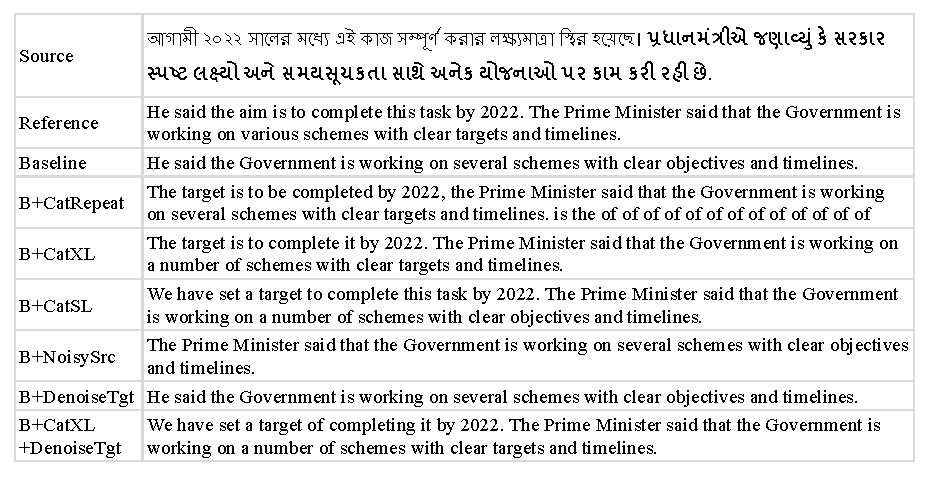
\includegraphics[width=0.98\linewidth,trim={2mm 2mm 2mm 2mm},clip]{img/robustness/example-translations.pdf}
    \caption{Example translations from the models trained on all-data setup.
    See Table~\ref{tab:bleu-alldata-augs} for quantitative scores of these models, and Figure \ref{fig:attnviz-catXL}  for a visualization of cross-attention.}
    \label{tab:fig:example-translations}
\end{table}
% and \ref{fig:attnviz-catXL+denoise}

\subsection{Attention Bleed}
\label{sec:attn-bleed}
% and \ref{fig:attnviz-catXL+denoise} 
Figure~\ref{fig:attnviz-catXL} visualizes cross-attention\footnote{Also known as encoder-decoder attention.} from our baseline model without augmentation as well as models trained with augmentation. 
Generally, the NMT decoder is run autoregressively; however, to facilitate the analysis described in this section, we force-decode reference translations and extract cross-attention tensors from all models.
%Since the sentence boundaries are required to determine the alignment of concatenated sentences,  we force-decode the reference translation that has known sentence boundaries.
The cross-attention visualization between a pair of concatenated sentences, say $(x_{i1} + x_{i2} \rightarrow y_{i1} + y_{i2})$, shows that models trained on augmented datasets appear to have less cross-attention mass across sentences, i.e., in the attention grid regions representing $x_{i2} \leftarrow y_{i1}$, and $x_{i1} \leftarrow y_{i2}$. 
We call attention mass in such regions \textit{attention bleed}. 
This observation confirms some of the findings suggested by \citet{nguyen-etal-2021-data}. 
We quantify attention bleed as follows: 
consider a Transformer NMT model with $L$ layers, each having $H$ attention heads and a held-out dataset of $\{(x_i ~ y_i) | i=1,2,...N\}$ segments. 
Furthermore, let each segment $(x_i, y_i) $ be a concatenation of two sentences, i.e. $(x_{i1}+ x_{i2}, ~ y_{i1}+y_{i2})$, with known sentence boundaries.
Let $|x_i|$ and $|y_i|$ be the sequence lengths after BPE segmentation, and $|x_{i1}|$ and $|y_{i1}|$ be the indices of the end of the first sentence (i.e., the sentence boundary) on the source and target sides, respectively.
%Therefore, the cross-attention tensor $A$ has the size $[ N x  L \times H \times |y_i| \times |x_i|]$.
% oops 5 dimensions will blew my mind. 
The average attention bleed across all the segments, layers, and heads is defined as:
$$ \bar{B} = \frac{1}{N \times L \times H} \sum_{i=1}^N \sum_{l=1}^L \sum_{h=1}^H b_{i,l,h}$$

\noindent where $b_{i,l,h}$ is the attention bleed rate in an attention head $h\in[1, H]$, in layer $l \in [1, L]$, for a single record at $i\in[1,N]$. 
To compute $b_{i,l,h}$, consider that an attention grid $A^{(i,l,h)}$ is of size $|y_i|\times|x_i|$. Then 
%Consider the attention bleed rate in an attention head $h\in[1, H]$ from layer $l \in [1, L]$, for a single record at $i\in[1,N]$. 
%The cross-attention grid $A$ is has the size of $|y_i|\times|x_i|$. 
%The attention bleed for segment $i$ in head $h$ at layer $l$ is given by $$
$$ b_{i,l,h} = \frac{1}{|y_i|} \Big[
      \sum_{t=1}^{|y_{i1}|} \sum_{s=|x_{i1}|+1}^{|x_i|} A^{(i,l,h)}_{t,s} 
    + \sum_{t=|y_{i1}|+1}^{|y_i|} \sum_{s=1}^{|x_{i1}|} A^{(i,l,h)}_{t,s} \Big] $$

%The average attention bleed across all the segments, layers, and heads as follows:
%$$ B = \frac{1}{N \times L \times H} \sum_{i=1}^N \sum_{l=1}^L \sum_{h=1}^H b_{i,l,h}$$

%%%%%%%%% COMMENT %%%%
\begin{comment}
Attention bleed rate for a single record $i$ having two concatenated sentences is given by:
\begin{multline*}
 B_i = \frac{1}{L \times H \times |y_i|} \sum_{l=1}^{L} \sum_{h=1}^{H} \bigg[ \sum A_{l,h}[y_{i1}, x_{i2}]\\ + \sum A_{l,h}[y_{i2}, x_{i1}] \bigg]
\end{multline*}
\noindent where $|y_i|$ is the number of tokens in the target sentence $y_{i1} + y_{i2}$ after BPE segmentation, $A[y_{i1}, x_{i2}]$ is the sum of attention paid by tokens in target sentence $y_{i1}$ to $x_{i2}$, and $A[y_{i2}:x_{i1}]$ is the sum of attention paid by target sentence $y_i2$ to $x_{i1}$. 
We compute average attention bleed across a corpus of $N$ such segments, as $$\bar{B} = \frac{1}{N} \sum_{i=1}^N B_i$$
\end{comment}
%%%%%%%%% COMMENT %%%%
\noindent where $A^{(i,l,h)}_{t,s}$ is the percent of attention paid to source position $s$ by target position $t$ at decoder layer $l$ and head $h$ in record $i$. Intuitively, a lower value of $\bar{B}$ is better, as it indicates that the model has learned to pay attention to appropriate regions. 
 As shown in Table~\ref{tab:xattn-bleed}, the models trained on augmented sentences achieve lower attention bleed. 

\begin{figure}[h!tb]
    %\includegraphics[width=2mm,angle=90,trim={24cm 1mm 0mm 35mm},clip]{attnviz-SL-baseline-xttn.png}
    \centering
    \begin{subfigure}[b]{0.49\linewidth}
        \centering
        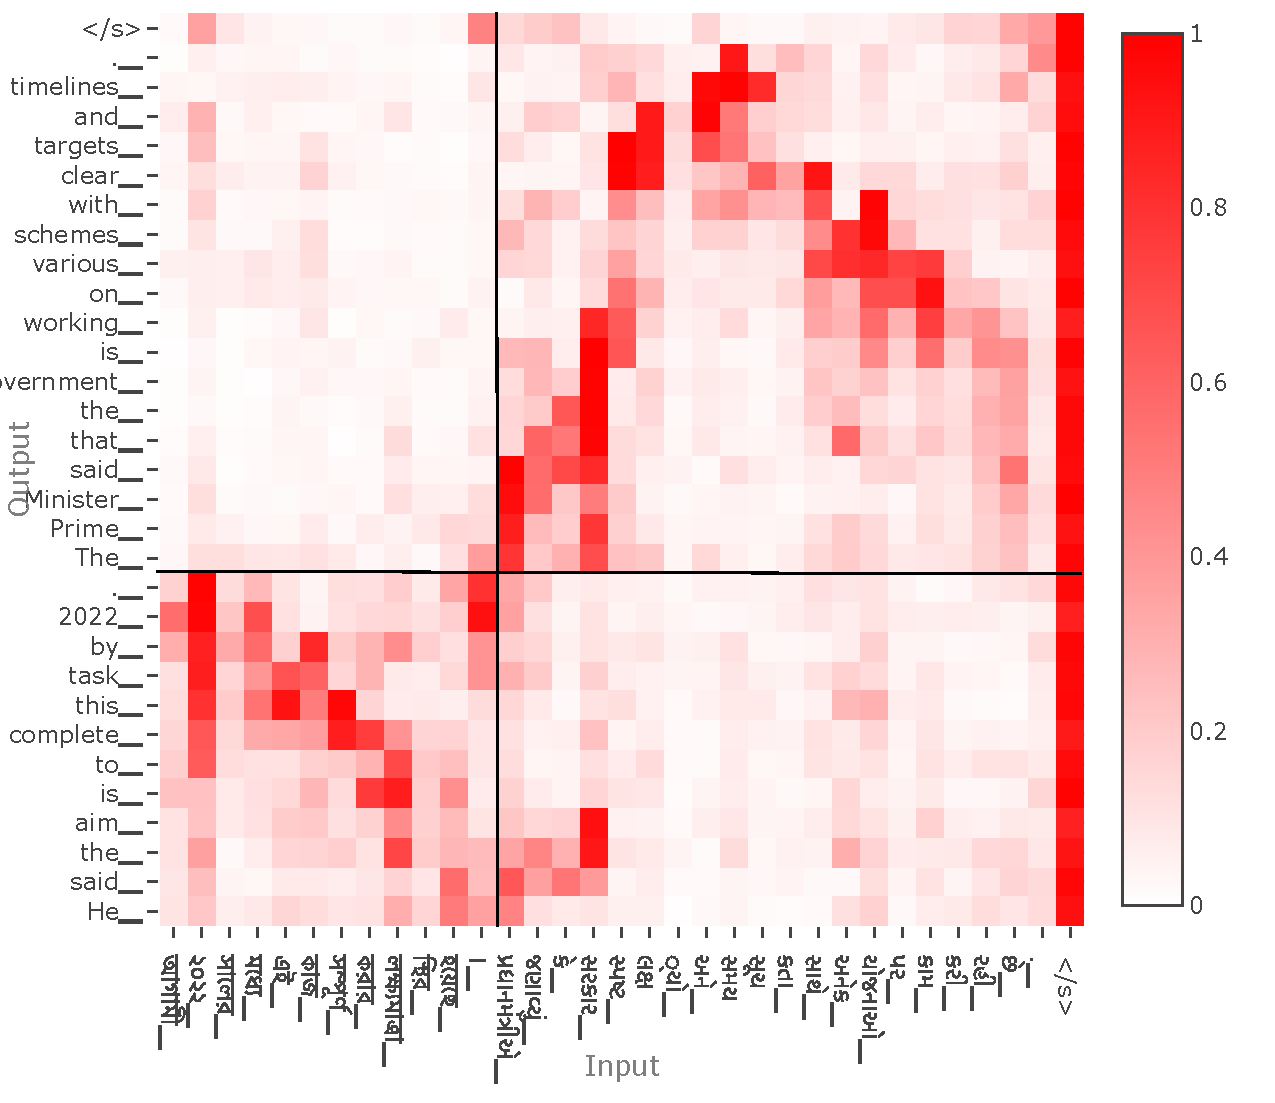
\includegraphics[width=\linewidth,trim={0mm 3mm 38mm 3mm},clip]{img/robustness/xattn-catXL-baseline-ann.pdf}
        \caption{Baseline without sentence concatenation (\#A1)}
        \label{fig:baseline-on-catXL}
     \end{subfigure}
    \begin{subfigure}[b]{0.49\linewidth}
        \centering
        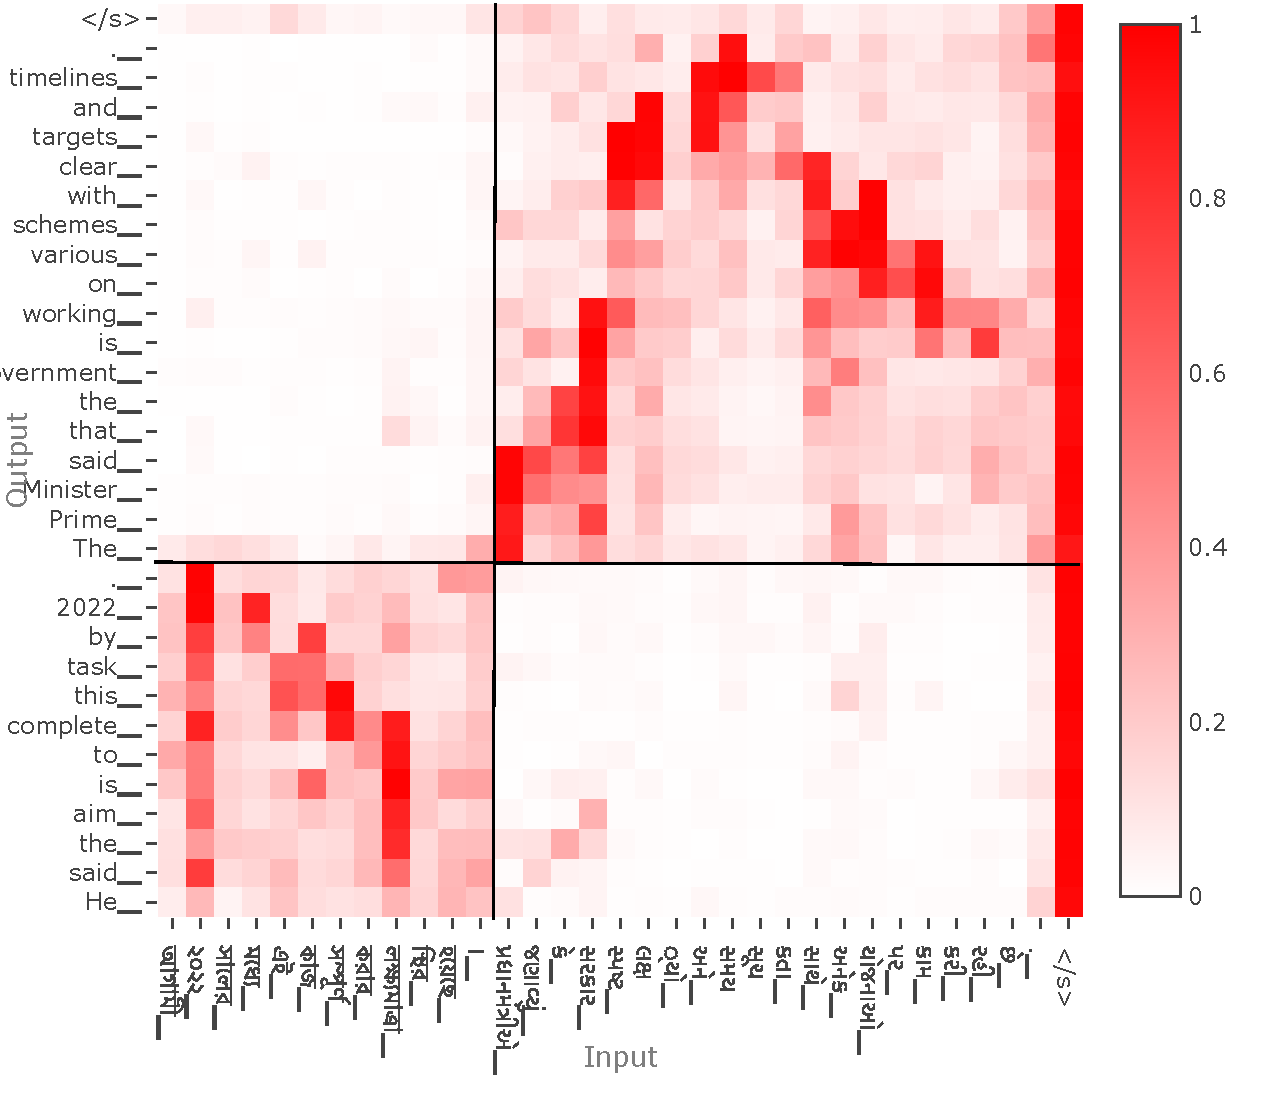
\includegraphics[width=\linewidth,trim={0mm 3mm 38mm 1mm},clip]{img/robustness/xattn-catXL-catXL-ann.pdf}
        \caption{Model trained with concatenated sentences (\#A3)}
        \label{fig:CatXL-on-CatXL}
     \end{subfigure}
   
   \vspace{5mm}
   
   \begin{subfigure}[b]{0.49\linewidth}
         \centering
         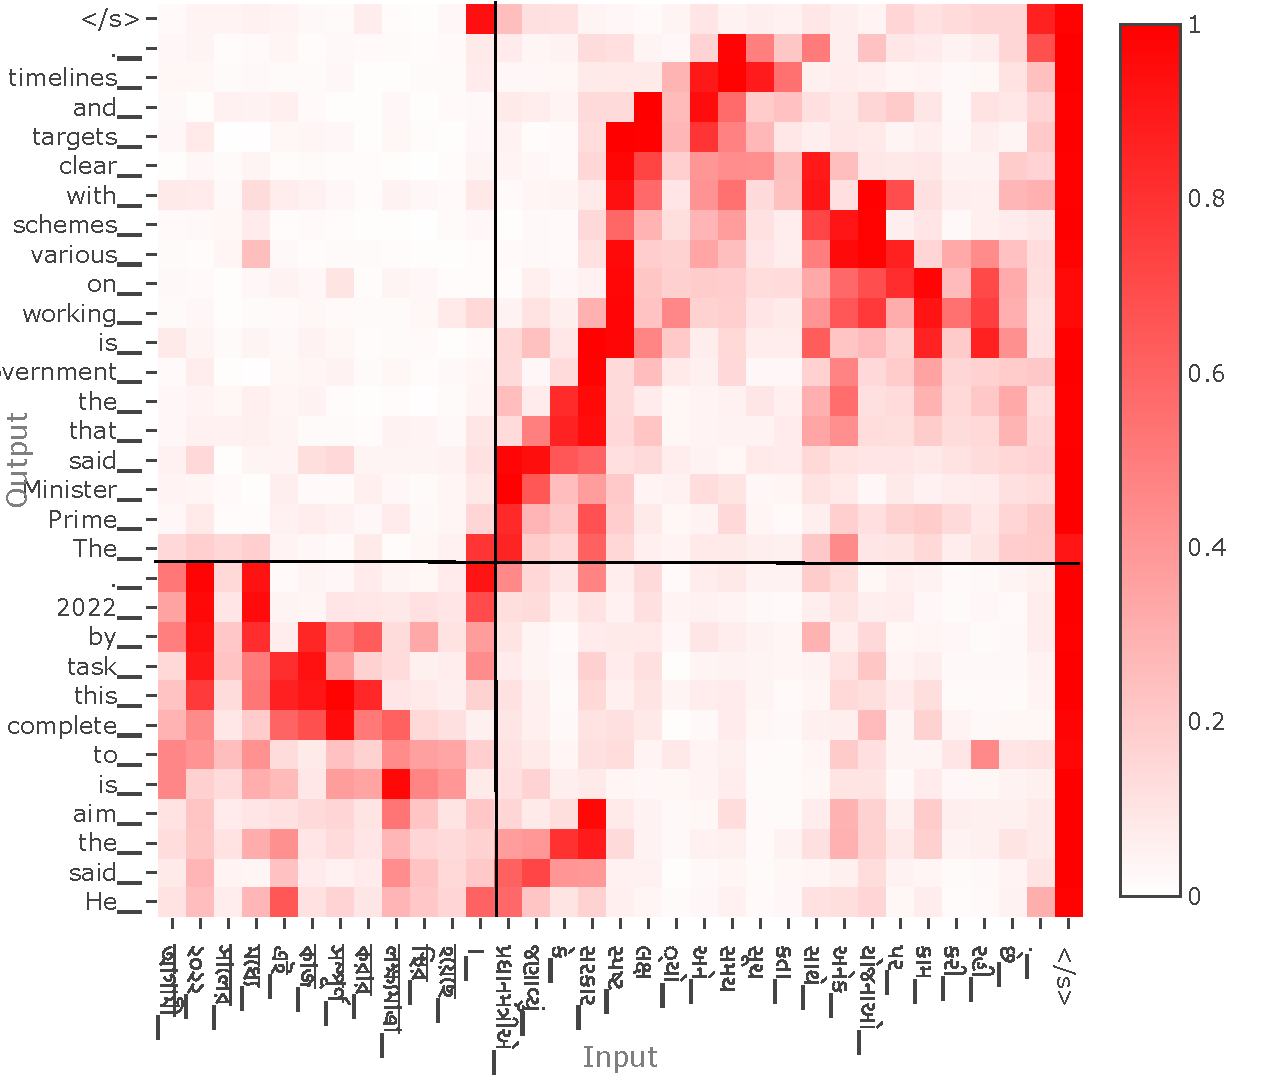
\includegraphics[width=\linewidth,trim={0mm 3mm 38mm 2mm},clip]{img/robustness/xattn-catXL-denoise-ann.pdf}
         \caption{Model trained with DenoiseTgt augmentation (\#A6)}
         \label{fig:denoise-on-catXL}
      \end{subfigure}
     \begin{subfigure}[b]{0.49\linewidth}
         \centering
         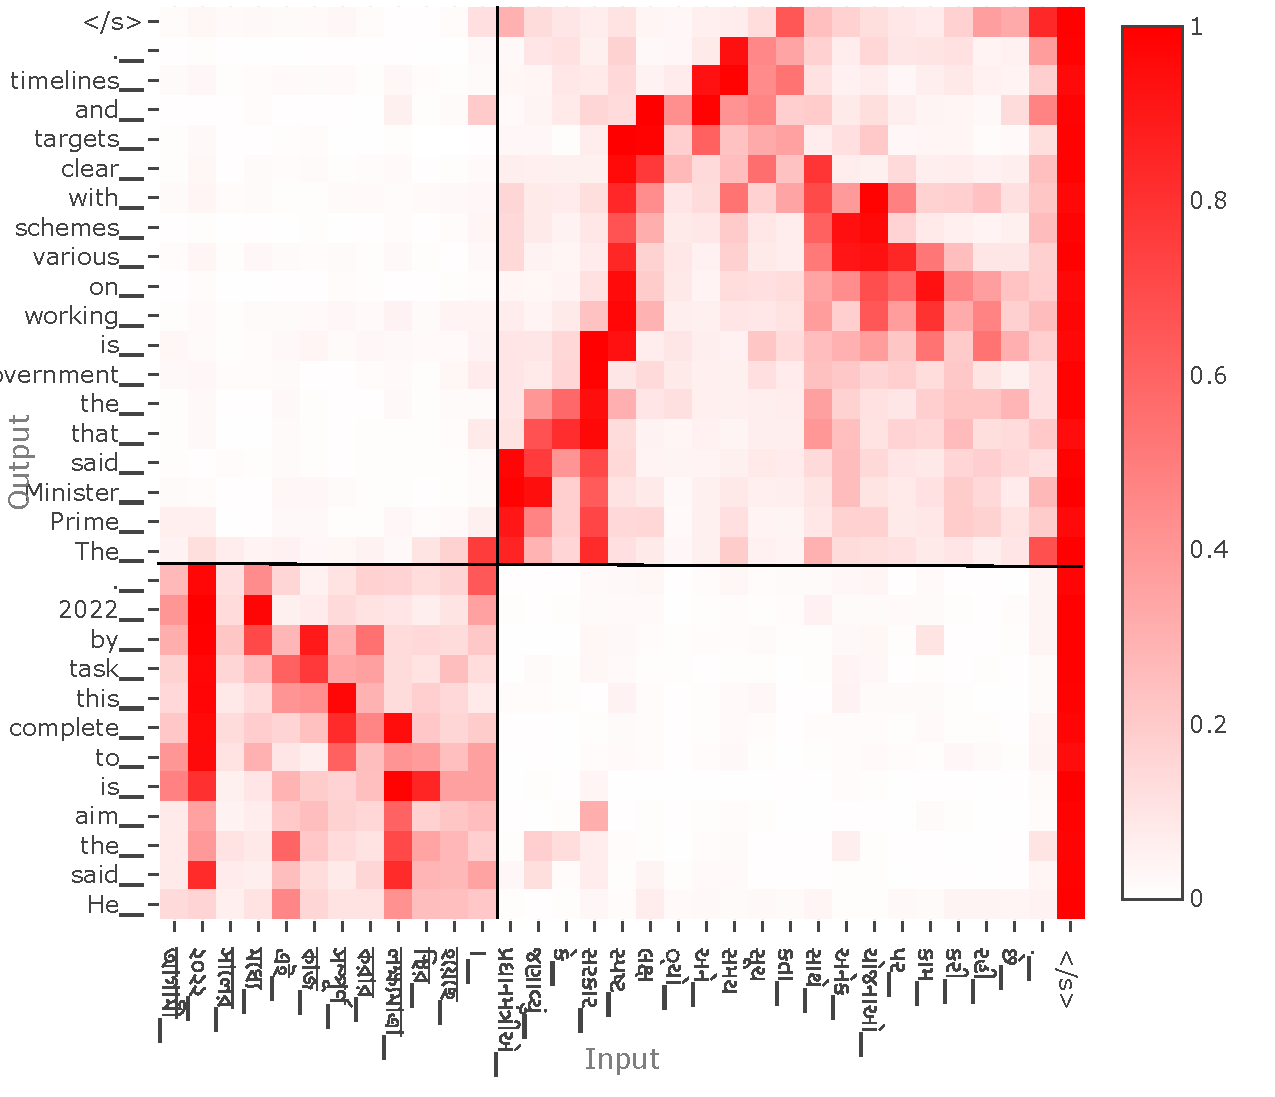
\includegraphics[width=\linewidth,trim={0mm 3mm 38mm 2mm},clip]{img/robustness/xattn-catXL-catXL+denoise-ann.pdf}
         \caption{Model trained with both CatXL and DenoiseTgt augmentations (\#A7)}
         \label{fig:denoise+catXL-on-catXL}
      \end{subfigure}
      
    \caption[Cross-attention visualization from baseline model and concatenated (cross-language) model.]{Cross-attention visualization from baseline model and concatenated (cross-language) model.
     For each position in the grid, only the maximum value across all attention-heads from all the layers is visualized. The darker color implies more attention weight, and the black bars indicate sentence boundaries. The model trained on concatenated sentences has more pronounced cross-attention boundaries than the baseline, indicating less mass is bled across sentences.
     The model trained on both concatenated and denoising sentences has the least attention mass across sentences.}
\label{fig:attnviz-catXL}
\end{figure}

\begin{comment}

\begin{figure}[h!t]
    \centering
    \begin{subfigure}[b]{0.49\linewidth}
         \centering
         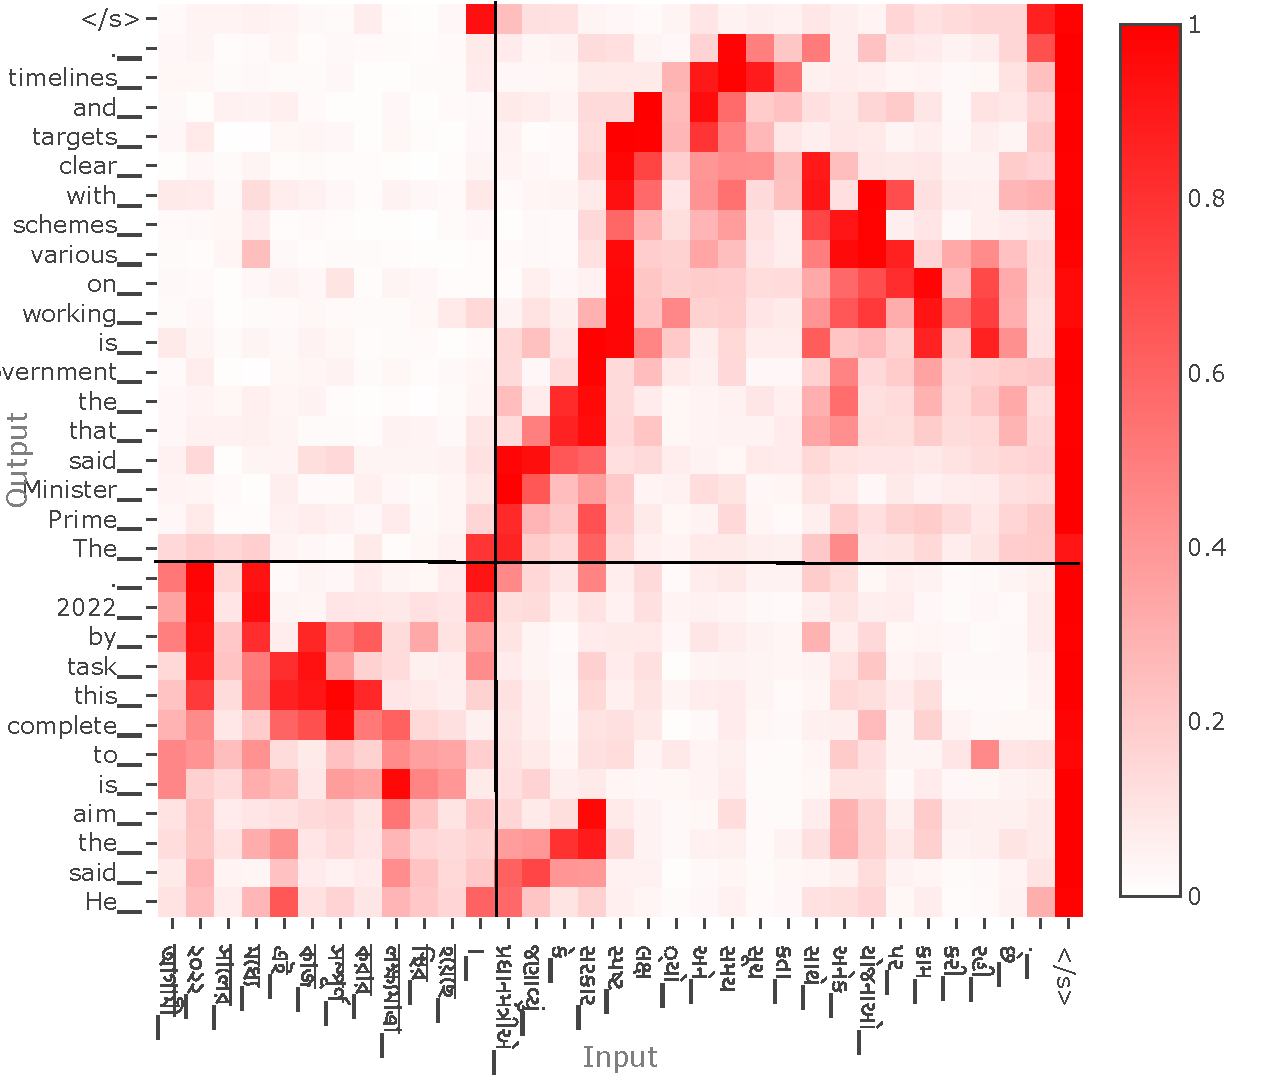
\includegraphics[width=\linewidth,trim={0mm 3mm 38mm 2mm},clip]{img/robustness/xattn-catXL-denoise-ann.pdf}
         \caption{Model trained with DenoiseTgt augmentation (\#A6)}
         \label{fig:denoise-on-catXL}
      \end{subfigure}
     \begin{subfigure}[b]{0.49\linewidth}
         \centering
         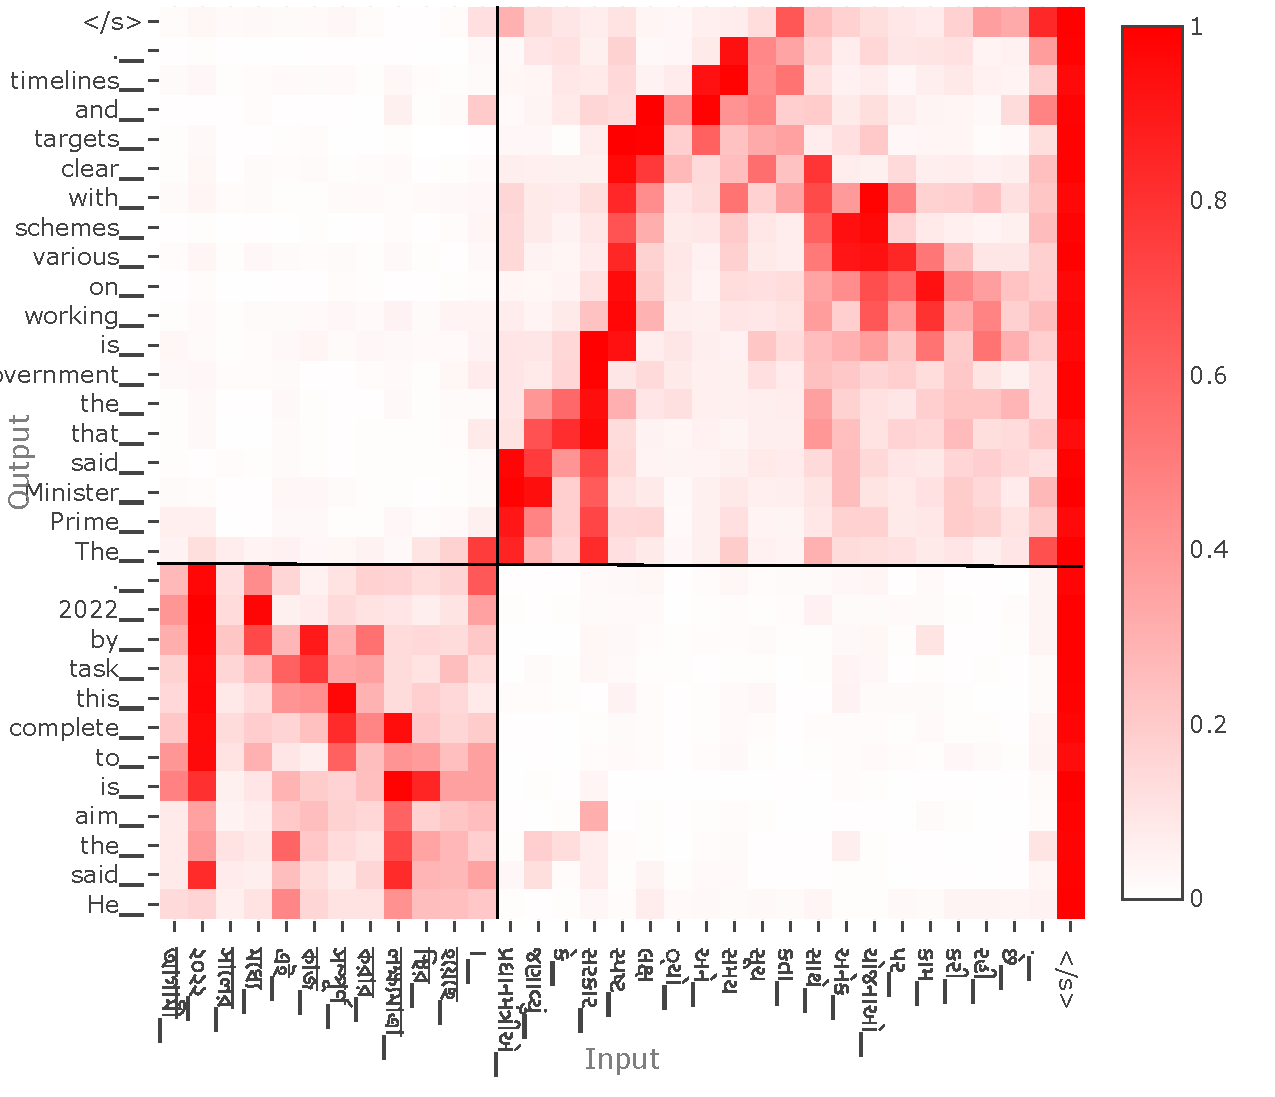
\includegraphics[width=\linewidth,trim={0mm 3mm 38mm 2mm},clip]{img/robustness/xattn-catXL-catXL+denoise-ann.pdf}
         \caption{Model trained with both CatXL and DenoiseTgt augmentations (\#A7)}
         \label{fig:denoise+catXL-on-catXL}
      \end{subfigure}
    \caption{Cross-attention visualization (... continuation from Figure~\ref{fig:attnviz-catXL}) The model trained on both concatenated and denoising sentences has least attention mass across sentences.}
    \label{fig:attnviz-catXL+denoise}
\end{figure}
\end{comment}
% test SVG support; oops fonts for unicodes are not supported
%\begin{figure}[htbp]
%  \centering
%  \includesvg[width=\linewidth]{tmp.svg}
%  \caption{svg image}
%\end{figure}


\subsection{Sentence Concatenation Generalization}
\label{sec:generalization}
In the previous sections, only two-segment concatenation has been explored; here, we investigate whether more concatenation further improves model performance and whether models trained on two segments generalize to more than two at test time.
We prepare a training dataset having up to four sentence concatenations and evaluate on datasets having up to four sentences.
As shown in Table~\ref{tab:cat-gen-bleus}, the model trained with just two segment concatenation achieves a similar BLEU as the model trained with up to four concatenations.
\begin{table}[ht]
\centering
\begin{tabular}{l rr : rr}
\hline
&\multicolumn{2}{c}{\textbf{Dev}} & \multicolumn{2}{c}{\textbf{Test}} \\
& C-SL & C-4SL & C-SL & C-4SL \\
\hline
Baseline / no join & 30.0 & 27.8 & 27.8 & 25.7 \\
Up to two joins & 31.9 & 28.9 & 29.7 & 26.7\\
Up to four joins & 31.0 & 28.9 & 28.8 & 26.8\\
\hline
\end{tabular} 
\caption{Indic$\shortarrow$English BLEU on held out sets containing up to 4 consecutive sentence concatenations in same language (C-4SL).
The two sentences dataset (C-SL) is also given for comparison.
The model trained on two concatenated sentences achieves comparable results on C-4SL, indicating that no further gains are obtained from increasing concatenation in training.}
\label{tab:cat-gen-bleus}
\end{table}


\section{Conclusion}

% We have investigated robustness of multilingual NMT and a few simple techniques to improve it.
We have described simple but effective checks for improving test coverage in multilingual NMT (Section~\ref{sec:multiling-mt-checks}), and have explored training data augmentation methods such as sentence concatenation and noise addition (Section~\ref{sec:train-aug}).
Using a many-to-one multilingual setup, we have investigated the relationship between these augmentation methods and their impact on robustness in multilingual translation. 
While the methods are useful in limited training data settings, their impact may not be visible on single-sentence test sets in a high resource setting. 
However, our proposed checklist evaluation reveals the robustness improvement in both the low resource and high resource settings.
We have conducted a glass-box analysis of cross-attention in Transformer NMT showing both visually and quantitatively that the models trained with augmentations, specifically, sentence concatenation and target sentence denoising, learn a more sharply focused attention mechanism (Section~\ref{sec:attn-bleed}).
Finally, we have determined that two-sentence concatenation in training corpora generalizes sufficiently to many-sentence concatenation inference (Section~\ref{sec:generalization}).  
%\section*{Acknowledgements}
%Thanks to 


\section*{Ethical Consideration}

%Machine translation is one of the very successful applications of natural language processing technologies, enabling communication across the language barriers.
%In this work we focus on a small subset of languages.

\paragraph{Limitations:} As mentioned in Section~\ref{sec:multiling-mt-checks}, some multilingual evaluation checks require the datasets to have multi-parallelism, and coherency in the sentence order.
When neither multi-parallelism nor coherency in the held-out set sentence order is available, we recommend R-XL. 
The data augmentation methods proposed in this paper do not require any specialized hardware or software.
Our model and training pipeline can be rerun on a variety of GPU models, including one with less memory, as 12 GB. 
However, some large dataset and large vocabulary models may require multiple distributed training processes, and/or multiple gradient accumulation steps to achieve the described batch size.

%\paragraph{Scientific Artifacts:} The experiments described in this chapter uses a dataset from The Workshop on Asian Translation 2021 (WAT21)'s \textit{MultiIndicMT} shared task~\cite{nakazawa-etal-2021-overview}, which is available for free download at the public URL: \url{http://lotus.kuee.kyoto-u.ac.jp/WAT/indic-multilingual/}; we do not redistribute this dataset from our servers.
%Our NMT pipeline is already publicly available under a license approved by \url{https://opensource.org}. Our code and scripts used for data preparation, augmentation, as well as model training and evaluation will be made available via a public GitHub repository with an open source-friendly license after the end of the author anonymity period. 

Only a subset of checks on robustness in multilingual settings have been discussed. While they serve as starting points for improving robustness, we do not claim that the proposed checks are exhaustive.
We have investigated robustness under Indic-English translation task where all languages use space characters as word-breakers; we have not investigated other languages such as Chinese, Japanese etc.
The term \textit{Indic} language to collectively reference 10 Indian languages only, similar to \textit{MultiIndicMT} shared task. While the remaining Indian languages and their dialects are not covered, 
we believe that the approaches discussed in this chapter generalize to other languages in the same family.
